En este laboratorio se busca analizar una muestra sanguínea mediante la técnica de AFM, y con los resultados conocer la morfología de las células conocidas como glóbulos rojos (eritrocitos).

\textbf{\textcolor{azul50}{Formalismo}}

La aplicación de un microscopio de fuerza atómica (AFM) para los trabajos en labratorio  ha proporcionado aumentar significativamente los conocimientos sobre las estructuras y procesos celulares. Este es un instrumento mecano-óptico capaz de detectar fuerzas del orden de los nanonewtons, el mismo es capaz de registrar continuamente su topografía mediante una sonda o punta afilada de forma piramidal o cónica, la sonda va acoplada a un listón o palanca microscópica muy flexible de sólo unos $200~\mu m$. El microscopio de fuerza atómica ha sido esencial en el desarrollo de la nanotecnología, para la caracterización y visualización de muestras a dimensiones nanométricas.

El AFM es una técnica tradicionalmente usada para mapear la topografía y estudiar las propiedades de materiales a escalas nanometricas, en esta se usa una punta tipo aguja en un extremo del cantilever para interactuar con el material (muestra). La interacción entre las muestras y la punta se manifiesta en fuerzas atractivas o repulsivas. Estas fuerzas brindan información sobre la topografía de la muestra. Si la punta y la muestra están cerca una de la otra, la fuerza de atracción trae la punta hacia la muestra, y cuando la punta es puesta en contacto con la muestra, la fuerza de repulsión rechaza a la punta lejos de la muestra. Este fenómeno puede ser
explicado por el principio de exclusión de Pauli. El cantilever actúa como el sensor de fuerza. Los cantilevers vienen en diferentes formas, la selección depende en el tipo de medición a la que será destinado. Con objeto de tener una sensibilidad pequeña a la fuerza, la masa del cantilever debe ser pequeña.

La aplicación del programa XEI para analizadar muestras proporcionadas por un equipo AFM es una práctica habitual ya que posee herramientas fáciles de usar y dinámicas para el procesamiento de imágenes, el análisis cualitativo y cuantitativo,
estadística, exportación e impresión de imágenes procesadas y resultados de las mediciones realizadas a las células sanguíneas, por eso es la herramienta que tradicionalmente se utiliza para ello por los investigadores ya que se convierte en la actualidad en una necesidad la caracterización de un
material con sus propiedades como las eléctricas,
mecánicas y químicas a escala nanométricas y de esta manera entender la naturaleza del
material.

La implementación de esta técnica en la investigación de los eritrocitos se considera algo habitual en el mundo científico, dadas las características de las células y lo munerosas que son en la sangre, mediante está técnica se ha podido constatar que los eritrocitos de los mamíferos, carecen de núcleo y de mitocondrias, además normalmente presentan forma oval, con una depresión en el centro mostrandose con una membrana con un espesor menor
a $0.1\%$ de la célula.

\textbf{\textcolor{azul50}{Procedimiento experimental}}

La muestra a estudiar fue el resultado de una extracción de sangre por medio de venopunción de un paciente, una gota de la misma fue colocada sobre una placa de vidrio  y una vez que se asegura que se distribuya de manera laminal a lo largo de la placa, se deja secar la misma por un tiempo aproximado de $10~min$, se procede entonces a la obtención de imagenes de los eritrocitos por AFM para su posterior análisis con XEI y matlab como programa alternativo para comparar resultados.

\textbf{Procesamiento con XEI y con matlab}

Para su procesamiento se hace necesario primeramente homogeneizar el fondo de la imagen, se sigue con la deteción de granos en la imagen, y obtención de los perfiles de superficies de cada grano detectado. Ya logrado esto se pasa a obtener las respectivas distribuciones correspondientes a los parámetros de células (diámetro medio $\overline{d}$ (considerandolos circulares), área de la superficie superior ($A$), perímetro de la célula en su vista superior ($P$), volumen total ($V$), valores de rugosidad superficial ($R_{vp}$ y $R_{rms}$), estos se visualizarán mediante sus respectivos histogramas. Finalmente se procederá a calcular los valores medio de estos parámetros con sus valores medios.

Se comparan los resultados obtenidos de forma independiente, valorando las fortalezas de cada estudio de forma independiente.

\textbf{\textcolor{azul50}{Obtención y análisis de Resultados}}

Se  procederá  a  analizar dos perfiles (ver Fig. \ref{original}) obtenidos al aplicar la técnica de AFM sobre una misma muestra.
\begin{figure}
    \centering
    %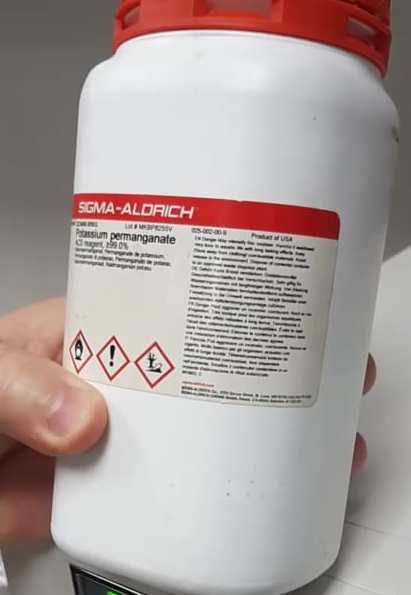
\includegraphics[width=0.3\textwidth]{Tarea1/muestras.png}
    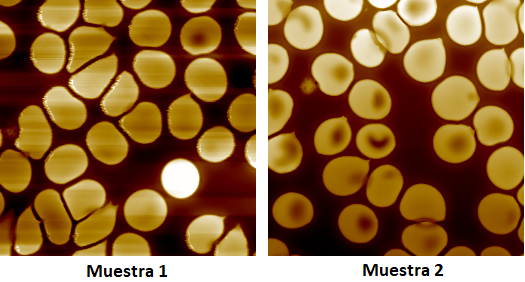
\includegraphics[width=0.49\textwidth]{Tarea4/muestras_originales.png}
    \caption{\textbf{Imagenes .tiff obtenidos con AFM.}}
    \label{original}
\end{figure}
Se utilizaron los programas XEI y matlab para procesar los perfiles, la renderización de los mismos se muestra en la Fig. \ref{perfil} mostrando claramente la presencia de elementos celulares bien definidos.
\begin{figure}
    \centering
    %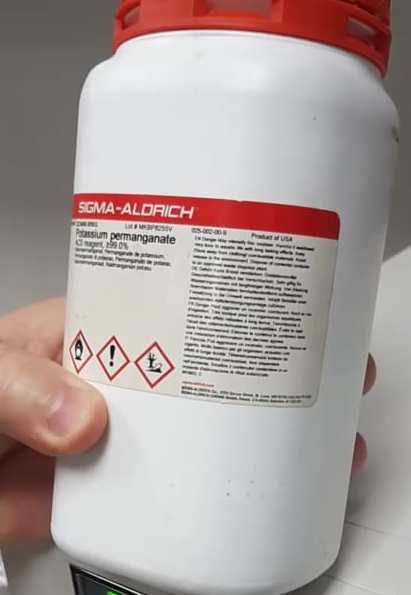
\includegraphics[width=0.3\textwidth]{Tarea1/muestras.png}
    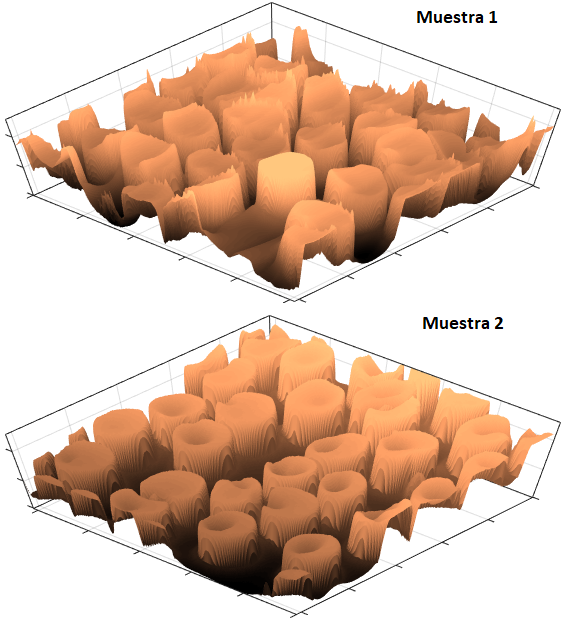
\includegraphics[width=0.49\textwidth]{Tarea4/perfil.png}
    \caption{\textbf{Gráficos 3D realizado en matlab de las muestras tratadas.}}
    \label{perfil}
\end{figure}
Se procedió inicialmente a homogeneizar la superficie de la muestra, este proceso es prácticamente automático con el XEI, pero en el caso del matlab se tuvo que primeramente recurrir por un proceso iterativo permitiendo mejorar significativamente el perfil resultante al despreciar las irregularidades superficiales del medio.
\textbf{\begin{figure}
    \centering
    %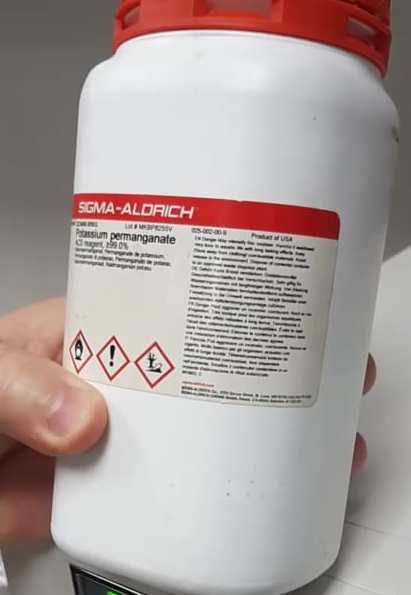
\includegraphics[width=0.3\textwidth]{Tarea1/muestras.png}
    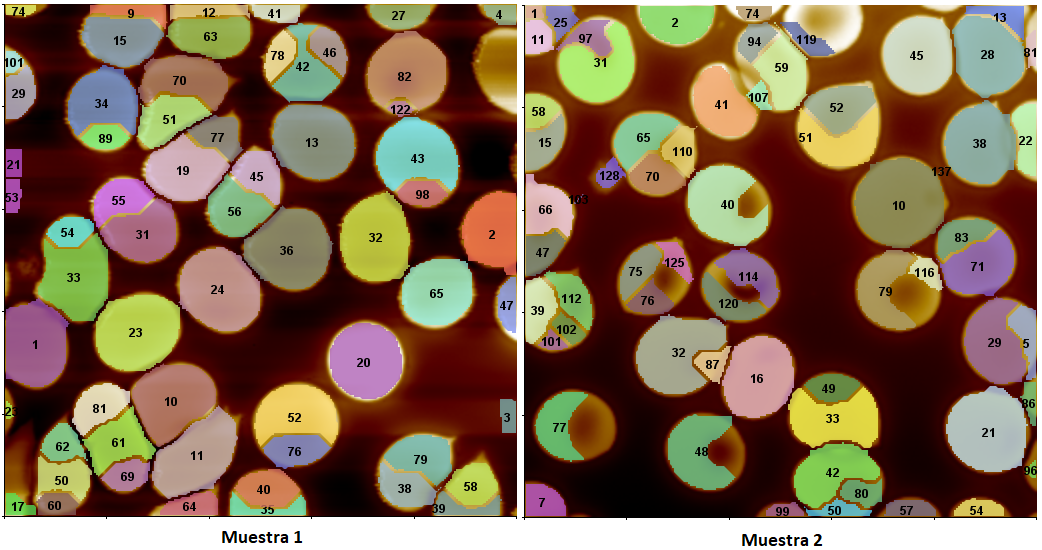
\includegraphics[width=0.49\textwidth]{Tarea4/XEI.png}
    \caption{\textbf{Procesamiento y localización de las objetos con XEI.}}
    \label{xei}
\end{figure}}
La identificación de los elementos en los perfiles se realiza de forma automática con el XEI (ver Fig. \ref{xei}), este identifica correctamente abruptos de gradiente en la imagen, como resultado de esto se localizarón efectivamente 229 elementos en las dos muestras mediante este programa, los errores posiblemente sean debido a una calibración errónea de los parámetros en el software introducidos por el usuario, esto disminuirá la fiabilidad de los resultados esperados. Para la identifiación de objetos realizado por el matlab se procedió con el aumento de contraste, la binarización y la identificación de objetos con redes neuronales (ver Fig. \ref{tratamiento}), se localizaron efectivamente 72 elementos, los resultados se muestran muy acordes con la comparación visual realizada a los perfiles originales.
\begin{figure}
    \centering
    %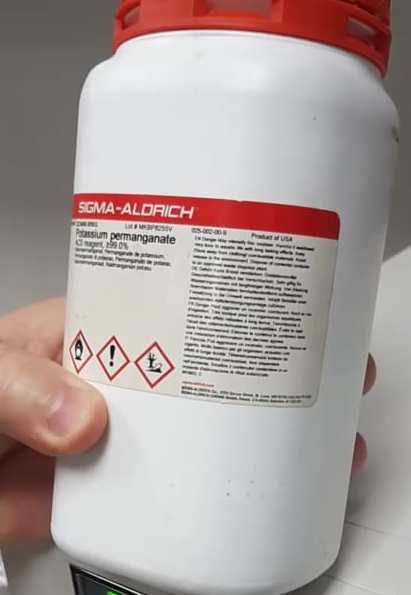
\includegraphics[width=0.3\textwidth]{Tarea1/muestras.png}
    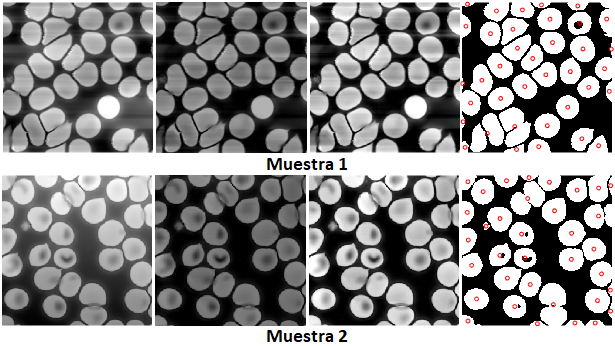
\includegraphics[width=0.49\textwidth]{Tarea4/tratamiento.png}
    \caption{\textbf{Procesamiento y localización de las objetos con matlab.}}
    \label{tratamiento}
\end{figure}
Se procede a la obtención de los parámetros celulares de interés ya explicados en la sección de procedimiento esperimental, la distribución de los mismos es visualizable en la Fig. \ref{histogramaprogram} para los resultados mostrados por XEI, y para el caso del matlab se procedió a la agrupación de parámetros correspondientes a las dos muestras, los mismos son mostrados en la Fig. \ref{histograma1}. 
\textbf{\begin{figure}
    \centering
    %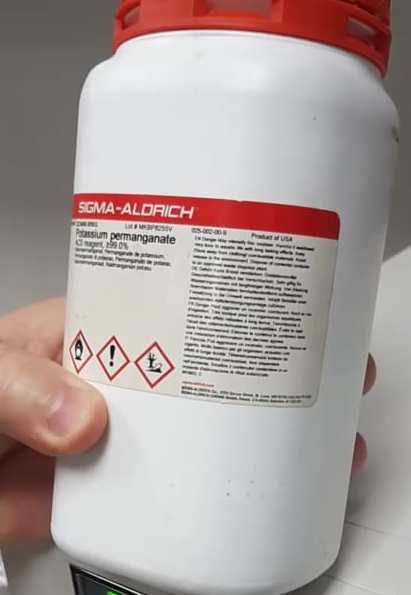
\includegraphics[width=0.3\textwidth]{Tarea1/muestras.png}
    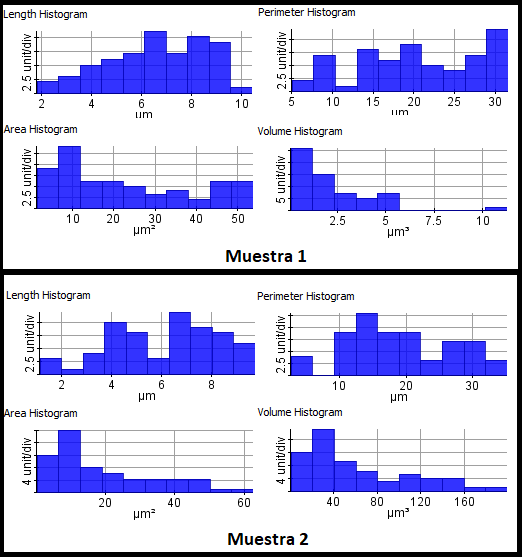
\includegraphics[width=0.49\textwidth]{Tarea4/histogramaprogram.png}
    \caption{\textbf{Histogramas de parámetros calculados por XEI.}}
    \label{histogramaprogram}
\end{figure}}
Al comparar la forma de las distribuciones se pudo constatar que hay correspondencia en los datos procesados por el XEI, pero las comparaciones con las distribuciones obtenidas con matlab muestra formas y agrupamientos inesperados, en especial en los parámetros correspondientes al área ($A$), volumen ($V$) y perímetro ($P$). Finalmente los párametros obtenidos se muestran en la Tabla 7.

\textbf{\begin{figure}
    \centering
    %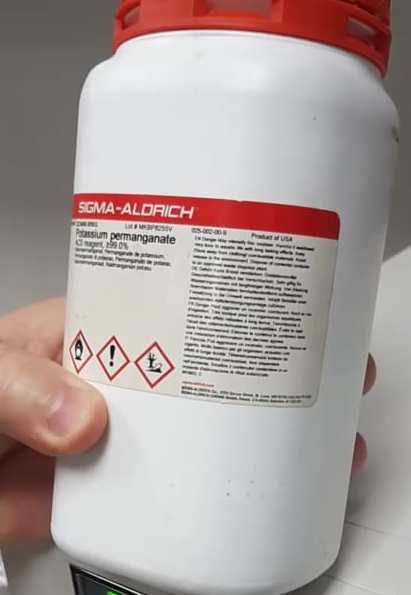
\includegraphics[width=0.3\textwidth]{Tarea1/muestras.png}
    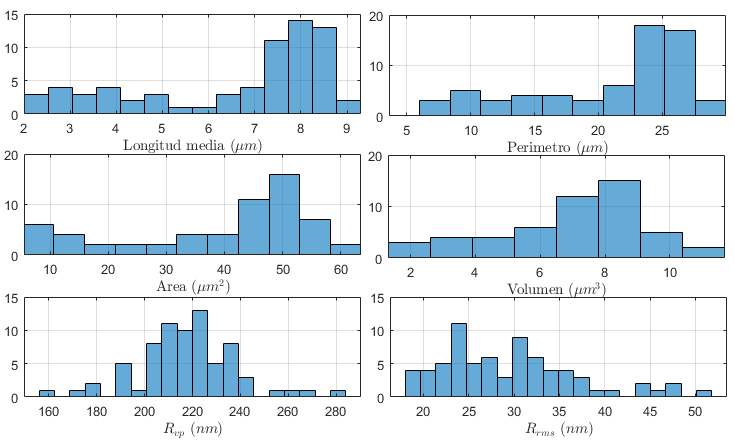
\includegraphics[width=0.49\textwidth]{Tarea4/histograma1.png}
    \caption{\textbf{Histogramas de parámetros calculados por matlab.}}
    \label{histograma1}
\end{figure}}
 
 \textbf{Tabla 7: Valores de los parámetros obtenidos al analizar las celulas con AFM.}
 
 \begin{tabular}{|c|c|c|c|}
    \hline
    Símbolo & XEI (media) & Matlab\\
    \hline
     $\overline{d}$ ($~\mu m$)& $6.584\pm 2.02$ & $6.88\pm 1.72$\\
     \hline
    $P$  ($\mu m$)& $20.36 \pm 7.466$ & $22.89\pm 9.04$  \\
     \hline
     $A$ ($\mu m^2$)& $22.48\pm 15.83$ &  $38.06\pm 22.92$ \\
     \hline
      $V$ ($\mu m^3$)&$2.13\pm 1.963$ & $8.73\pm 1.25$  \\
     \hline
     ($R_{pv}$) (nm)& $293.20\pm 103.39$  & $220.78\pm 51.21$\\
     \hline
\end{tabular}

Al comparar los resultados obtenidos en la tabla, se pudo observar cierta correpondencia de los mismos, aunque los valores de $A$ y $V$ para el XEI se muestran irreales.

\textbf{\textcolor{azul50}{Conclusiones}}

Con el procesamiento de los perfiles reportados por el equipo AFM de los globulos rojos mediante dos métodos alternativos, y con una leve comparación de los resultados se da por cumplido el objetivo del laboratorio.
